\subsection{Aerodynamic Performance Analysis [Andy McClaskey]}
\paragraph{Aerodynamic Reference Area}
The reference area needed for calculated lift and drag was determined by assuming a trapezoidal wing planform. The root and tip chord length were used as inputs to the area equation to calculate the wing planform area. The equation used for calculation total wing area is shown in Equation \ref{eqn:aeroRefArea}.

\begin{equation}
\label{eqn:aeroRefArea}
S = (\text{Root Chord} + \text{Tip Chord})*\frac{\text{Wing Span}}{2}
\end{equation}

The planform was optimized for a drag to help increase the lift to drag ratio later in the design

\paragraph{Drag Determination}

The Coefficient of Drag ($C_D$) was taken from the 1x scale Generic Hypersonic Vehicle \cite{ghv} for the angle of attack of zero. Once the coefficient of drag was known, the total drag could be calculated using Equation \ref{eqn:drag}. They dynamic pressure is known from the free stream conditions of the vehicle and the aero reference area is known from above. The Coefficient of Drag is plotted in Figure \ref{fig:CdVMach}.

\begin{equation}
\label{eqn:drag}
D = q_{\infty}SC_D
\end{equation}

\begin{wrapfigure}{r}{0.65\textwidth}
\begin{center}
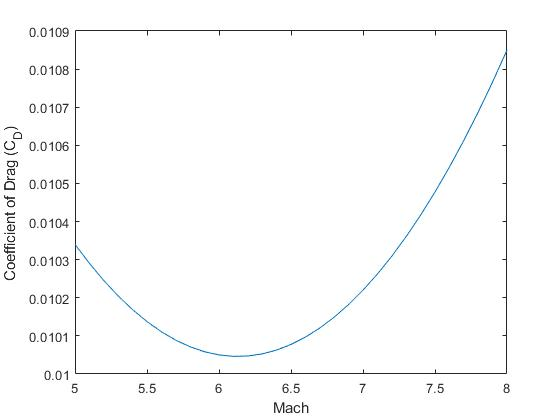
\includegraphics[width=0.6\textwidth]{CdVMach}
\caption{$C_D$ v. Mach}
\label{fig:CdVMach}
\end{center}
\end{wrapfigure}

\begin{comment}
The total drag for the vehicle is shown in Figure \ref{fig:dragVMach}.

\begin{wrapfigure}{r}{0.65\textwidth}
\begin{center}
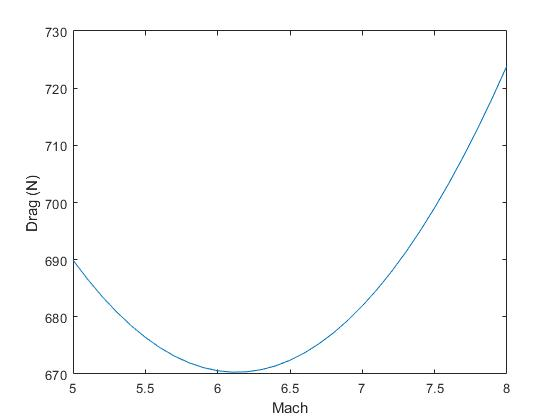
\includegraphics[width=0.6\textwidth]{dragVMach}
\caption{Drag v. Mach}
\label{fig:dragVMach}
\end{center}
\end{wrapfigure}

\end{comment}

\paragraph{Thrust Required}
The drag determined above sets the thrust required from the propulsion system for the vehicle in straight and level unaccelerated cruise flight.
For the acceleration part of the mission the thrust required is shown in Equation \ref{eqn:thrustRequired}. It was assumed that the pitch angle was close to zero for this analysis.

\begin{equation}
\label{eqn:thrustRequired}
\text{Thrust}=m\frac{dv}{dt}+D+mg\sin{\theta}
\end{equation}

\paragraph{Lift Determination}
In the cruise portion of the mission, the weight of the vehicle is known, we can determine the Coefficient of Lift required to support the vehicle. This is done using Equation \ref{eqn:liftCoef}.

\begin{equation}
\label{eqn:liftCoef}
C_L=\frac{\text{weight}}{q_{\infty}S}
\end{equation}

\paragraph{Lift over Drag}
The Lift to Drag Ratio is calculated using Equation \ref{eqn:LtoD}. Lift over drag is a primary input into the Bergeut range equation that can be used later for estimating the range. The Lift to Drag ratio is plotted in Figure \ref{fig:ClCdVMach}. The drag was optimized to be at its minimum at our cruise condition. With more time, the component build up method could be used to determine if this drag estimate is accurate.

\begin{equation}
\label{eqn:LtoD}
\text{Lift over Drag} = \frac{C_L}{C_D}
\end{equation}

\begin{figure}[H]
\begin{center}
\includegraphics[width=0.6\textwidth]{ClCdVMach}
\caption{$C_L/C_D$ v. Mach}
\label{fig:ClCdVMach}
\end{center}
\end{figure}